% TECHNICAL_REPORT.tex
% Compile with: pdflatex TECHNICAL_REPORT.tex  (run twice for the table of contents)
% Only standard TeX Live / MiKTeX packages are used.

\documentclass[11pt,a4paper]{article}

\usepackage[T1]{fontenc}
\usepackage[utf8]{inputenc}
\usepackage{lmodern}
\usepackage{microtype}
\usepackage[margin=2.5cm]{geometry}
\usepackage{booktabs}
\usepackage{tabularx}
\usepackage{longtable}
\usepackage{array}
\usepackage{amsmath}
\usepackage{graphicx}
\usepackage{xcolor}
\usepackage{enumitem}
\usepackage{fancyhdr}
\usepackage{caption}
\usepackage{listings}
\usepackage{tikz}
\usetikzlibrary{arrows.meta,positioning,fit,backgrounds}
\usepackage[hidelinks]{hyperref}

\definecolor{accent}{RGB}{176,32,86}
\definecolor{codebg}{RGB}{246,246,248}
\definecolor{codekw}{RGB}{20,80,160}
\definecolor{codecm}{RGB}{110,110,110}
\definecolor{boxline}{RGB}{130,130,140}

\lstset{
  basicstyle=\ttfamily\small,
  backgroundcolor=\color{codebg},
  keywordstyle=\color{codekw}\bfseries,
  commentstyle=\color{codecm}\itshape,
  stringstyle=\color{accent},
  numbers=left,
  numberstyle=\tiny\color{codecm},
  numbersep=8pt,
  frame=single,
  rulecolor=\color{boxline},
  breaklines=true,
  showstringspaces=false,
  captionpos=b,
  xleftmargin=16pt,
  columns=fullflexible,
}

\captionsetup{font=small,labelfont=bf}

\pagestyle{fancy}
\fancyhf{}
\fancyhead[L]{\small Foodpanda Karachi Ordering Assistant}
\fancyhead[R]{\small\thepage}
\renewcommand{\headrulewidth}{0.4pt}

\newcommand{\code}[1]{\texttt{\small #1}}

% Let TeX stretch a stubborn line instead of pushing it into the margin.
\setlength{\emergencystretch}{2em}

\begin{document}

%% ---------------------------------------------------------------- title page
\begin{titlepage}
\centering
\vspace*{1.2cm}

{\Huge\bfseries Foodpanda Karachi Ordering Assistant\par}
\vspace{0.5cm}
{\LARGE A Grounded Conversational Agent over a\\[2pt] Scraped Restaurant Snapshot\par}
\vspace{0.4cm}
{\large Architecture, Data Pipeline, and Verified Implementation Status\par}

\vspace{1.4cm}

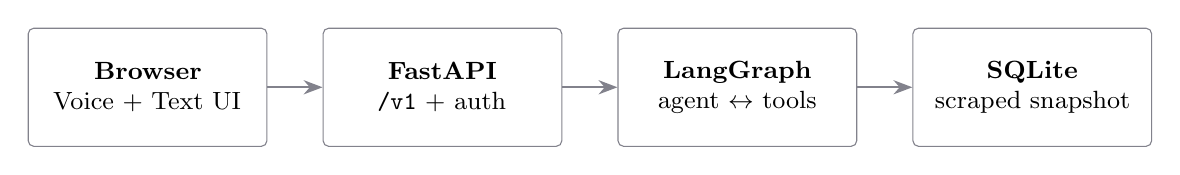
\begin{tikzpicture}[
  every node/.style={font=\small},
  box/.style={draw=boxline, rounded corners=2pt, align=center,
              minimum height=1.5cm, text width=2.75cm, inner sep=4pt},
  arr/.style={-{Stealth[length=2.4mm]}, draw=boxline, thick}
]
\node[box] (a) {\textbf{Browser}\\Voice + Text UI};
\node[box, right=0.7cm of a] (b) {\textbf{FastAPI}\\\code{/v1} + auth};
\node[box, right=0.7cm of b] (c) {\textbf{LangGraph}\\agent $\leftrightarrow$ tools};
\node[box, right=0.7cm of c] (d) {\textbf{SQLite}\\scraped snapshot};
\draw[arr] (a) -- (b);
\draw[arr] (b) -- (c);
\draw[arr] (c) -- (d);
\end{tikzpicture}

\vspace{1.4cm}

{\large\bfseries Technical Project Report\par}
\vspace{0.25cm}
{\large Milestones 1, 5 and 6 implemented and verified\par}

\vspace{1.0cm}

{\normalsize Built with Python, LangGraph, FastAPI, SQLite,\\
Google Gemini, Groq (Whisper / Orpheus)\par}

\vfill
{\large Ameer Hamza\par}
\vspace{0.2cm}
{\large Software Engineering Internship Project\par}
\vspace{0.3cm}
{\large August 25, 2026\par}
\end{titlepage}

%% ------------------------------------------------------------------ abstract
\section*{Abstract}
\addcontentsline{toc}{section}{Abstract}

This report documents a conversational food-ordering assistant built over a
scraped snapshot of Foodpanda Pakistan restaurant data for Karachi. The system
holds a natural conversation until the user knows what to order: it draws out
craving, area, party size and budget, recommends restaurants ranked by a
review-weighted rating rather than raw stars, searches a single locked
restaurant's menu, assembles a cart, and prepares an order summary. Every
factual claim the assistant makes --- restaurant, dish, price, rating,
delivery estimate --- must originate in a tool result read from the snapshot;
the model is explicitly forbidden from supplying any of them from its own
parametric knowledge. The assistant does \emph{not} place orders and does not
track deliveries, because Foodpanda exposes no public API for either.

The report is deliberately weighted toward what has been built and verified.
Milestone~1 (chat), Milestone~5 (voice) and Milestone~6 (multi-tenant API
service layer) are implemented and evidenced by automated tests and live
runs. Milestone~2 (daily live scraping) is fully implemented and unit-tested
but has \textbf{never completed a live run against the real database}, and is
reported as such rather than as operational. Milestone~3 is only partially
addressed through a manually curated review sample, and Milestone~4 has not
been started. All quantitative claims in this document are traceable to a
recorded measurement in the repository's engineering notes or to a
verification performed while writing this report.

\vspace{0.35cm}
\noindent\textbf{Keywords:} LangGraph, ReAct agents, tool calling, grounded
generation, web API scraping, SQLite, Bayesian shrinkage ranking, FastAPI,
API-key authentication, rate limiting, multi-tenancy, speech interfaces.

\vspace{0.6cm}
{\small\itshape Verification basis: row counts, migration state and the test
suite result quoted throughout were re-run on 27~August~2026 against the live
repository, not copied from earlier documentation.}

\clearpage
\tableofcontents
\clearpage

%% ------------------------------------------------------------------ 1 summary
\section{Executive Summary}

The product is a chat-and-voice ordering assistant for Foodpanda Pakistan
restaurants in Karachi, aimed at a diner who knows they are hungry but has not
decided where to order from. It converses until the order is decided,
recommends specific dishes with real prices and ratings drawn from a scraped
SQLite snapshot, and produces a labelled order summary that the user carries
to the Foodpanda app to actually check out. It is exposed as a versioned,
authenticated HTTP service with per-key rate limiting and usage metering, so
it can be consumed by any client rather than only by the bundled demo page.

Current state: the conversational core, the voice layer and the API service
layer are complete and verified; the daily re-scraping scheduler is written
and unit-tested but has never published a live refresh; deals and scraped
review text were not built, and order-status tracking was never started.
Table~\ref{tab:milestones} is the authoritative status view.

\begin{table}[htbp]
\centering
\caption{Milestone status. ``Verified'' means an automated test or a recorded
live run exists; ``built, unverified live'' means code and unit tests exist but
the real end-to-end path has never been exercised.}
\label{tab:milestones}
\small
\begin{tabularx}{\textwidth}{@{}l l X@{}}
\toprule
\textbf{Milestone} & \textbf{Status} & \textbf{Evidence / caveat} \\
\midrule
1 --- Chat assistant & Done, verified &
Tools, ranking, policy grounding, in-memory sessions; covered by the automated
suite and by live tool-level runs. \\
\addlinespace
2 --- Daily live scraping & \textbf{Built, never run live} &
Scheduler, migration and 16 unit tests exist. \code{scrape\_runs} holds
\textbf{0} rows and \textbf{0} of 209 restaurants have ever been refreshed. The
schedule is not enabled. \\
\addlinespace
3 --- Deals \& reviews & Partial & Deals \textbf{not built}. Review
\emph{text} is not exposed by the Foodpanda APIs; a \textbf{manual} sample of
107 reviews across 23 restaurants was imported instead. \\
\addlinespace
4 --- Order status & Not started &
Requires the user's own authenticated Foodpanda session; out of reach of
generic scraping. \\
\addlinespace
5 --- Voice layer & Done, verified &
Push-to-talk Whisper STT, server-side Orpheus TTS with 200-character chunking
and WAV concatenation. Agent graph untouched. \\
\addlinespace
6 --- API service layer & Done, verified &
API-key auth, tenant isolation, rate limiting, usage metering, \code{/v1}
versioning. Verified by unit tests plus live HTTP runs. \\
\bottomrule
\end{tabularx}
\end{table}

\noindent
Two figures anchor the rest of this report. The snapshot currently holds
\textbf{209 restaurants, 1{,}671 menu categories and 12{,}224 menu items} with
\textbf{zero} rows failing the standing broken-price diagnostic, and the
automated suite currently reports \textbf{140 tests, all passing}. Both were
re-measured on 27~August~2026 for this document.

%% ------------------------------------------------------------- 2 architecture
\section{Architecture Overview (Implemented)}

The system is three cooperating layers over one read-only data file: a
LangGraph agent that reasons and calls tools, a FastAPI service that
authenticates and meters requests, and a SQLite snapshot that is the only
source of factual content. A provider router sits behind the model call so
capacity failures at one LLM vendor do not surface as errors to the caller.

\subsection{The LangGraph Agent Loop}

The agent is a ReAct-style loop compiled as a two-node LangGraph state graph:
an \emph{agent} node that calls the model, and a \emph{tools} node that
executes whatever the model requested. Control alternates between them and the
loop terminates when the model answers without requesting a tool. A recursion
limit of 25 steps bounds a runaway loop while still allowing roughly a dozen
tool calls in one turn, since each tool call costs two graph steps.

Conversation state is a \code{TypedDict} carried by the graph and persisted by
a checkpointer keyed on the session:

\begin{lstlisting}[language=Python,caption={Conversation state (agent/state.py, abridged).}]
class OrderState(TypedDict, total=False):
    messages: Annotated[list, add_messages]
    location: str | None
    restaurant_id: int | None
    restaurant_name: str | None
    party_size: int | None
    craving: str | None
    budget: float | None          # total order budget in PKR
    deal_sensitive: bool | None
    cart: list[dict]              # [{item_id, name, price, qty}]
    order_summary: dict | None
    showcase: dict | None         # photo cards for the current turn
\end{lstlisting}

Nine tools are registered, and they are the only permitted source of factual
claims (Table~\ref{tab:tools}). Restaurant search and menu search are
deliberately separate tools rather than one parametrised tool: a session locks
exactly one restaurant, and separating them lets the menu and cart tools
hard-fail before a lock exists instead of trusting the model to respect a
\code{restaurant\_id} argument. It also keeps the reasoning trace readable.

\begin{table}[htbp]
\centering
\caption{The nine registered tools.}
\label{tab:tools}
\small
\begin{tabularx}{\textwidth}{@{}l X@{}}
\toprule
\textbf{Tool} & \textbf{Responsibility} \\
\midrule
\code{remember\_preferences} & Persist craving, party size, budget, location and deal-sensitivity as they emerge. \\
\code{search\_restaurants} & Match craving against cuisine, name, then dish names; rank by relevance tier, then weighted rating; return review counts and a confidence flag. \\
\code{get\_reviews} & Return stored review text for a named restaurant; returns \code{AMBIGUOUS} with candidates rather than guessing a branch. \\
\code{lock\_restaurant} & Lock one restaurant; refuses to switch without \code{confirm\_switch=True}, and clears the cart on a confirmed switch. \\
\code{search\_menu} & Search the locked restaurant's menu only; relaxes price and category filters before returning nothing. \\
\code{add\_to\_cart} / \code{remove\_from\_cart} / \code{view\_cart} & Cart mutation and inspection, validated against the locked restaurant. \\
\code{confirm\_order} & Build the order summary through the same function the HTTP confirm route uses. \\
\bottomrule
\end{tabularx}
\end{table}

A subtlety that turned into a real defect (Section~\ref{sec:parallel}) is that
the model may emit \emph{parallel} tool calls in one graph step. State keys
therefore carry explicit reducers: \code{showcase} merges within a step and
replaces across steps, \code{cart} is written as composable deltas rather than
whole-list replacements, and scalar preference keys resolve last-write-wins.

\subsection{The FastAPI Layer}

Every functional route lives under a \code{/v1} prefix and requires an API key;
\code{/health}, \code{/docs} and the demo page stay public. The routes are
listed in Table~\ref{tab:routes}.

\begin{table}[htbp]
\centering
\caption{HTTP contract. All \code{/v1} routes require a key.}
\label{tab:routes}
\small
\begin{tabularx}{\textwidth}{@{}l X@{}}
\toprule
\textbf{Endpoint} & \textbf{Purpose} \\
\midrule
\code{POST /v1/sessions} & Issue an unguessable session identifier. \\
\code{POST /v1/chat} & One conversational turn: \code{\{session\_id, message\}} $\rightarrow$ \code{\{reply, state\}}. \\
\code{POST /v1/chat/stream} & The same turn delivered as server-sent token events. \\
\code{POST /v1/sessions/\{id\}/location} & Browser coordinates $\rightarrow$ resolved Karachi area. \\
\code{POST /v1/sessions/\{id\}/welcome} & Opening line, computed without a model call. \\
\code{GET /v1/sessions/\{id\}/cart} & Current cart, item count and subtotal. \\
\code{POST /v1/sessions/\{id\}/confirm} & Order summary object. \\
\code{POST /v1/voice/transcribe} & Multipart audio $\rightarrow$ transcript plus latency. \\
\code{POST /v1/voice/speak} & Text $\rightarrow$ a single WAV body. \\
\code{GET /v1/usage} & The caller's own request and token totals. \\
\code{GET /health} & Model and snapshot readiness; no key required. \\
\bottomrule
\end{tabularx}
\end{table}

The checkpointer is the single source of truth for a session. The cart and
confirm routes read the same store the agent writes, so the HTTP view cannot
drift from what the conversation believes. Sessions live in process memory and
are lost on restart --- an accepted limitation, not an oversight
(Section~\ref{sec:limits}).

\subsection{The SQLite Data Layer}

The agent opens the scraped snapshot read-only, with a short-lived connection
per tool call. It never writes: cart and order state live in the checkpointer,
not in the database file. That posture is deliberate, because the daily
refresh republishes the whole file by atomic replacement.

Four tables carry the snapshot --- \code{restaurants}, \code{menu\_categories},
\code{menu\_items} and \code{scrape\_runs} --- plus a \code{reviews} table for
the manually imported sample. Current contents, queried directly for this
report on 27~August~2026, are shown in Table~\ref{tab:rows}.

\begin{table}[htbp]
\centering
\caption{Live snapshot contents, measured 27 August 2026.}
\label{tab:rows}
\small
\begin{tabular}{@{}l r@{}}
\toprule
\textbf{Quantity} & \textbf{Value} \\
\midrule
Restaurants & 209 \\
Menu categories & 1{,}671 \\
Menu items & 12{,}224 \\
Restaurants with zero menu items & 0 \\
Rows failing the broken-price diagnostic & 0 \\
Manually imported reviews & 107 \\
Restaurants covered by those reviews & 23 \\
Rows recorded in \code{delivery\_areas} as Gulshan-e-Iqbal & 87 \\
Rows recorded in \code{delivery\_areas} as Gulistan-e-Jauhar & 58 \\
Rows with no recorded \code{delivery\_areas} & 64 \\
Restaurants ever refreshed by the daily job & \textbf{0} \\
Rows in \code{scrape\_runs} & \textbf{0} \\
\bottomrule
\end{tabular}
\end{table}

A note on data types worth stating plainly: \code{menu\_items.price} is stored
as \code{TEXT} and parsed with a cast at query time. That is inherited from the
original scraper schema, and it is the reason the standing broken-price
diagnostic (Section~\ref{sec:dealbug}) is a text-pattern query rather than a
numeric one.

\subsection{LLM Provider Routing}

The default configuration uses Google Gemini \code{gemini-3.1-flash-lite} as
the primary chat model with Groq \code{openai/gpt-oss-20b} as a fallback. This
is a capacity decision, not a quality preference, and it was made in response
to a measured failure rather than pre-emptively.

During latency instrumentation, a single \code{/chat} turn took 28{,}886~ms
wall clock, of which one LLM round accounted for 25{,}492~ms. The cause was
not a slow model but a client-side back-off: the Groq SDK was silently
retrying after 24 seconds because the free-tier \emph{tokens-per-day} quota
(200{,}000) had been exhausted. Once identified, the response was to route
around capacity rather than to attempt to optimise it away. Both clients are
constructed with \code{max\_retries=0} so a 429 fails immediately instead of
the SDK sleeping; a Gemini 429 starts a process-wide cooldown and the same
turn retries Groq; if both providers fail, the graph commits a friendly
assistant message instead of raising.

The router is deliberately placed \emph{behind} \code{get\_llm()} and exposes
the same chat-model interface, so the graph, tools and prompts never branch on
provider. Both providers already normalise to the same message representation
with a uniform tool-call list, which is what makes the substitution safe
mid-conversation.

\subsection{Request Flow}

\begin{enumerate}[itemsep=2pt,topsep=4pt]
\item The client sends \code{\{session\_id, message\}} with an API key.
\item Auth resolves the tenant; the session is namespaced as
      \code{tenant:session\_id} before it ever reaches the graph.
\item The agent node rebuilds the system prompt from current state --- role
      rules, the extracted platform-policy text, and a digest of what the
      session already knows --- and calls the model.
\item Requested tools execute in the tool node. State-changing tools return a
      command so that the state update and the tool message land together.
\item Steps 3--4 repeat until the model replies without a tool call. After the
      first tool round the prompt is swapped for a much smaller routing prompt
      (Section~\ref{sec:latency}).
\item The API returns \code{\{reply, state\}}, and metering is written after
      the response body completes.
\end{enumerate}

\begin{figure}[htbp]
\centering
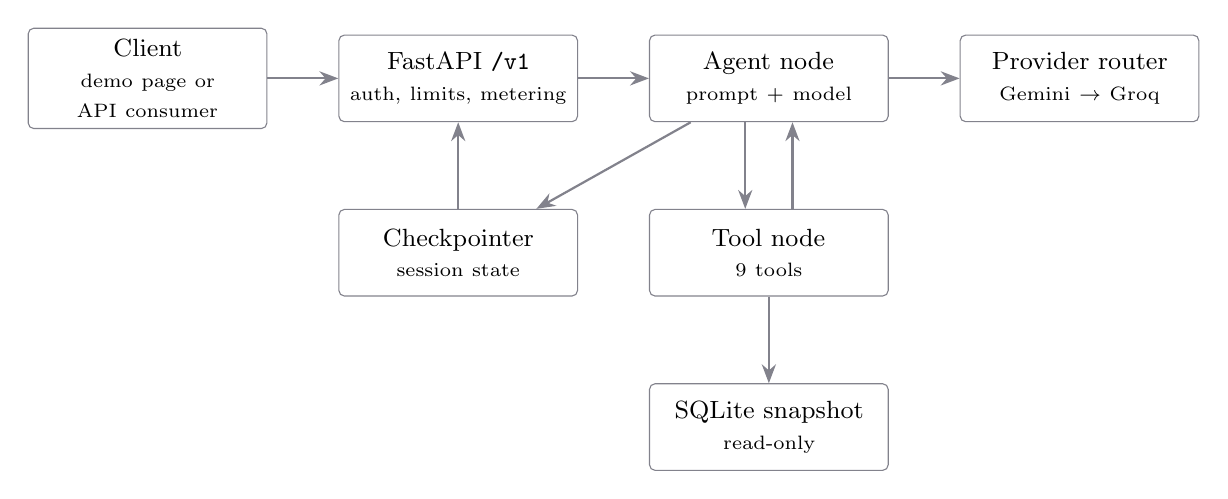
\begin{tikzpicture}[
  every node/.style={font=\small},
  box/.style={draw=boxline, rounded corners=2pt, align=center,
              minimum height=1.1cm, text width=2.75cm, inner sep=4pt},
  arr/.style={-{Stealth[length=2.4mm]}, draw=boxline, thick},
  lab/.style={font=\scriptsize, midway}
]
\node[box] (client) {Client\\\scriptsize demo page or API consumer};
\node[box, right=0.9cm of client] (api) {FastAPI \code{/v1}\\\scriptsize auth, limits, metering};
\node[box, right=0.9cm of api] (agent) {Agent node\\\scriptsize prompt + model};
\node[box, below=1.1cm of agent] (tools) {Tool node\\\scriptsize 9 tools};
\node[box, right=0.9cm of agent] (llm) {Provider router\\\scriptsize Gemini $\rightarrow$ Groq};
\node[box, below=1.1cm of api] (saver) {Checkpointer\\\scriptsize session state};
\node[box, below=1.1cm of tools] (db) {SQLite snapshot\\\scriptsize read-only};

\draw[arr] (client) -- (api);
\draw[arr] (api) -- (agent);
\draw[arr] (agent) -- (llm);
\draw[arr] ([xshift=-3mm]agent.south) -- ([xshift=-3mm]tools.north);
\draw[arr] ([xshift=3mm]tools.north) -- ([xshift=3mm]agent.south);
\draw[arr] (tools) -- (db);
\draw[arr] (agent) -- (saver);
\draw[arr] (saver) -- (api);
\end{tikzpicture}
\caption{Request flow for one conversational turn. The agent and tool nodes
alternate until the model answers without requesting a tool. Only the tool
node touches the snapshot, and it opens it read-only.}
\label{fig:flow}
\end{figure}

%% ------------------------------------------------------------- 3 data pipeline
\section{Data Pipeline (Implemented)}

\subsection{Why API Calls Rather Than Browser Scraping}

Navigating \code{www.foodpanda.pk} with a headless browser is blocked by
PerimeterX and reCAPTCHA: pages return ``Access to this page has been denied''
and no data requests fire at all. Rather than fight the bot protection, the
scraper targets the same internal JSON endpoints the site's own front end
uses, which answer plain HTTP requests without a browser session when the
correct hosts and headers are supplied.

Listings come from the Delivery Hero discovery service:

\begin{lstlisting}[caption={Listing endpoint. \texttt{sort=rating\_desc} reproduces the site's ``Top rated'' ordering.}]
GET https://disco.deliveryhero.io/listing/api/v1/pandora/vendors
    ?latitude=24.8607&longitude=67.0011&country=pk
    &vertical=restaurants&limit=48&offset=0
    &sort=rating_desc&language_id=1&include=characteristics
Header: x-disco-client-id: web
\end{lstlisting}

Menus come from the per-vendor endpoint, which additionally requires two
pseudo-session headers; without them it returns
\code{HTTP 400 \{"error":"perseus headers are absent"\}}:

\begin{lstlisting}[caption={Menu endpoint and its required headers.}]
GET https://pk.fd-api.com/api/v5/vendors/{code}
    ?latitude={lat}&longitude={lng}&language_id=1&include=menus
Headers: X-FP-API-KEY: volo
         Referer / Origin: https://www.foodpanda.pk
         perseus-client-id / perseus-session-id: <pseudo ids>
\end{lstlisting}

Three practical constraints were discovered by measurement and shape the whole
pipeline. First, the listing feed only returns vendors that are currently open
and accepting orders, so scrape timing materially changes what is collected.
Second, the menu endpoint returns an \emph{empty} menu when the queried
coordinates fall outside a vendor's delivery zone, so requests must use the
area centre that discovered the vendor rather than one city-wide point. Third,
the menu host will start returning PerimeterX 403 responses under sustained
probing; the scrapers therefore rotate the user agent, sleep 1.5--3.0 seconds
between every request, and abort the menu phase after five consecutive 403s
rather than deepening a live block.

\subsection{Dataset Size and Coverage}

The snapshot was assembled in three passes, none of which re-identified or
mutated rows from an earlier pass. An original Karachi scrape produced 29
restaurants. A well-known expansion then queried 11 area centres, keeping only
vendors with at least 3{,}208 reviews --- the dataset median at the time,
chosen deliberately so that ``well known'' meant the same thing as the ranking
model's shrinkage parameter. A final additive pass covered Gulshan-e-Iqbal and
Gulistan-e-Jauhar, taking the snapshot from 64 restaurants and 4{,}241 menu
items to \textbf{209 restaurants and 12{,}224 menu items}, with the original 29
identifiers untouched.

Coverage is recorded per row in a \code{delivery\_areas} column that stores the
\emph{discovery pin area} rather than the street address. That distinction was
forced by real data: a restaurant addressed in Bahadurabad may nonetheless
deliver to the Gulshan pin, so a street address is where the kitchen sits, not
where the food can go. As Table~\ref{tab:rows} records, 64 rows still carry no
delivery area, all of them from the two pre-column batches.

\subsection{Review-Weighted Ranking}

Sorting by star rating alone is misleading on this dataset. Review volume
spans roughly three orders of magnitude, from 18 to 39{,}949 reviews, so a
5.0 backed by 63 reviews sits directly above a 4.9 backed by 39{,}949. The
ranking layer therefore applies IMDB-style Bayesian shrinkage toward the
dataset mean:

\begin{equation}
\text{weighted\_rating} \;=\; \frac{v}{v+m}\,R \;+\; \frac{m}{v+m}\,C
\end{equation}

\noindent where $R$ is the restaurant's rating, $v$ its review count, $m$ the
dataset median review count and $C$ the dataset mean rating. Both $m$ and $C$
are recomputed at query time --- currently $m = 3{,}208$ and $C \approx
4.807$ --- so a later re-scrape changes the ranking without any code change.

Two honest caveats are carried in the implementation rather than hidden.
First, shrinkage is \emph{symmetric}: it lifts bad-with-few-reviews as much as
it demotes good-with-few-reviews, which is why the agent is required to cite
the review count alongside any rating and to hedge explicitly when a rating is
flagged low-confidence. Second, weighted scores across the top restaurants sit
within roughly 0.005 of each other, so ranking on that score alone let a
19{,}935-review chain outrank an actual specialist; relevance to the stated
craving is therefore tiered \emph{first}, and the weighted rating breaks ties
inside a tier.

\subsection{Review Text: A Manual Sample, Not Scraped}

Review \emph{text} is not obtainable from these APIs. The listing feed exposes
a \code{review\_with\_\allowbreak comment\_number} field that is \textbf{0} for every
vendor observed, so there is no comment payload to collect. Rather than
fabricate the feature, a bounded manual sample was used: review text for 23
Gulistan-e-Jauhar-area restaurants was copied by hand from the Foodpanda app
and imported into a \code{reviews} table, yielding \textbf{107 rows across 23
restaurants} (re-verified for this report). Reviewer names are not stored, the
import is idempotent, and liked-dish mentions are resolved to menu item
identifiers where a match exists. The agent surfaces these through
\code{get\_reviews} and is instructed never to invent sentiment or paraphrase a
review it did not receive. This is a sample, not city-wide coverage, and it is
labelled that way in the data (\code{source = manual\_sample}).

%% --------------------------------------------------------- 4 implementations
\section{Implementations}

\subsection{Milestone 1 --- The Conversational Assistant}

\subsubsection*{What it does}

One user talks to one session. The assistant establishes the Karachi area
first, because the listing data is delivery-scoped and recommending across the
city would be meaningless; it then draws out craving, party size, budget and
deal-sensitivity through conversation rather than a form. It recommends
restaurants, locks exactly one, searches that restaurant's menu, builds a cart
with itemised totals, and finally produces an order summary. Platform
questions --- delivery fees, cancellation, vouchers --- are answered from an
extract of Foodpanda's real Terms and FAQ pages, not from model memory; if
that extract is missing, the assistant is instructed to refuse rather than
guess.

\subsubsection*{How grounding is enforced}

Grounding is enforced in three places at once, because prompt instructions
alone are not a guarantee. The system prompt states that every restaurant,
dish, price, rating and delivery estimate must come from a tool result in the
current conversation. The tool layer is the only code path that reads the
database, so there is no way for the model to obtain a fact except through a
tool. And the tools return structured, cited values --- ratings always
accompanied by review counts and a confidence flag --- so a compliant reply
carries its own evidence. Cart totals add a delivery fee and a platform fee,
which are flat constants (99.0 and 8.99 PKR) recorded from an observation of
the listing feed rather than read per restaurant, and they are presented as
typical checkout extras rather than as a live quote.

\subsubsection*{Evidence it works}

\begin{itemize}[itemsep=3pt,topsep=4pt]
\item \textbf{Full-path wiring, without model spend.} A scripted stub model
      drives a complete session --- preferences, search, lock, menu, cart,
      confirm --- and then exercises the HTTP contract. This proves graph
      wiring, state updates and endpoint behaviour deterministically; it
      explicitly does \emph{not} evaluate conversation quality.
\item \textbf{Area search, live.} After the Gulshan/Jauhar import, the query
      ``chai in Jauhar'' returned 15 restaurants where it had previously
      returned 2, and area coverage rose from 2 rows to 62
      (Section~\ref{sec:areabug}).
\item \textbf{Multi-item ordering, live.} The request ``2 parathas and 3 cup
      chai'' completed in 6 tool rounds, \textbf{4 of them parallel},
      producing a final cart of Sada Paratha $\times$2 and Special Doodh Patti
      Chai $\times$3, subtotal 477 and total 584.99, with both card sets
      retained (Section~\ref{sec:parallel}).
\item \textbf{Restaurant name resolution, live.} A \code{get\_reviews} retest
      showed ``pizza day night'' with a Jauhar location returning 4 reviews for
      the correct row, the same query \emph{without} a location correctly
      returning \code{AMBIGUOUS} across branches instead of guessing, and a
      single-token query returning \code{NO\_MATCH} rather than a false
      positive.
\end{itemize}

\subsection{Milestone 5 --- The Voice Layer}

\subsubsection*{What it does and how}

Voice is strictly additive: the agent graph, conversation state and tool logic
were not modified. Interaction is push-to-talk with no wake word and no
always-on microphone. The user records, the audio is posted to a transcription
route backed by Whisper (\code{whisper-large-v3-turbo}), and the transcript is
placed \emph{into the input box rather than sent}. That deliberate pause
exists because dish names and prices are exactly the tokens speech recognition
gets wrong, and an unreviewed transcript would silently corrupt an order.

Text-to-speech runs on the server, not in the browser. The Orpheus model
accepts at most 200 characters per request, so replies are split by a
dedicated chunker and the resulting WAV clips are concatenated into a single
audio body at a pinned sample rate. Keeping that on the server means the
browser never learns about the character cap, and playback is one audio
element with no inter-chunk click. The chunker is careful about the tokens
that matter here: it will not split \code{Rs.} away from its number, and it
prefers sentence then clause boundaries before falling back to spaces. Speech
never blocks text --- the reply is painted first, and audio is a second
request that is skipped entirely when the user has muted output.

\subsubsection*{Evidence}

The chunker is pure logic with no I/O and is unit-tested on its own, including
the money-token and long-sentence cases. The transcription route's failure
modes are covered in the smoke test: a request with no file is rejected as
unprocessable, empty audio returns a client error, and an oversized upload is
rejected rather than forwarded. Latency is measured server-side and returned
to the caller in the response body and headers, so it is observable rather
than assumed.

\subsubsection*{One recent, unverified change}

The transcription call was recently changed to pin the recognition language to
Urdu with a mixed Urdu/English priming prompt, because auto-detection was
transcribing Urdu speech as Hindi in Devanagari script. This change is
\textbf{not covered by an automated test and has not been confirmed by a
recorded live run}; it is listed as an open item in
Section~\ref{sec:limits} rather than claimed as working.

\subsection{Milestone 6 --- The Multi-Tenant API Service Layer}

\subsubsection*{What it does}

This milestone wrapped the existing contract with authentication, per-key rate
limiting, usage metering, tier configuration and \code{/v1} versioning. It is
a wrapper, not a redesign: request and response shapes were preserved. No new
runtime dependencies were added --- key generation, hashing and storage all use
the standard library.

\subsubsection*{Authentication and key storage}

Keys are 256-bit random strings displayed exactly once at creation; only a
SHA-256 hash is stored, so a lost key is reissued rather than recovered. The
choice of a fast hash over a slow key-derivation function is deliberate and
worth defending, because ``hash it'' usually implies bcrypt or argon2: slow
KDFs exist to make dictionary attacks on \emph{low-entropy human passwords}
expensive. These keys are high-entropy random tokens where dictionary attack
is not a threat model, and a slow hash would add tens of milliseconds to every
API call while forcing a full table scan, since a salted slow hash cannot be
looked up by index. A short non-secret prefix is stored in the clear purely so
logs and dashboards can identify a key without revealing it.

Enforcement is a FastAPI dependency rather than blanket middleware, which
keeps the health check, documentation and demo page public while every
\code{/v1} route requires a key, and makes the security scheme appear
correctly in the generated OpenAPI document.

\subsubsection*{Tenant isolation by construction}

The security finding that shaped this milestone is described in
Section~\ref{sec:tenant}. The resolution was to namespace the session key with
the tenant identifier so that cross-tenant access is not merely checked but
\emph{unrepresentable}.

\subsubsection*{Rate limiting and metering}

Two independent limits apply per key, deliberately stored differently because
they fail differently. The per-minute burst limit is an in-memory token
bucket, where losing state on restart is harmless. The daily quota lives in
SQLite, because a quota that resets whenever the process restarts is not a
quota. Limits themselves are data, not code (Table~\ref{tab:tiers}), so
changing them is a configuration edit; an unknown tier name fails loudly at
startup rather than silently defaulting to something generous.

\begin{table}[htbp]
\centering
\caption{Tier limits, loaded from configuration at startup.}
\label{tab:tiers}
\small
\begin{tabular}{@{}l r r r@{}}
\toprule
\textbf{Tier} & \textbf{Per minute} & \textbf{Per day} & \textbf{Burst} \\
\midrule
\code{free} & 20 & 100 & 10 \\
\code{pro} & 120 & 10{,}000 & 60 \\
\code{unlimited} & 600 & 1{,}000{,}000 & 200 \\
\bottomrule
\end{tabular}
\end{table}

Every authenticated request writes one metering row --- route, status,
latency, and prompt/completion token counts when a model actually ran ---
rolled up per key per UTC day. Metering never breaks a request: a failure to
record usage is logged and swallowed. Tenant data is stored in a
\emph{separate} SQLite file from the scraped snapshot, for a specific
cross-milestone reason: the daily scrape copies the snapshot to a sidecar,
works for roughly 25 minutes, then atomically replaces the original, so
anything written to the snapshot during that window would be silently
destroyed by the swap. Billing rows that vanish for 25 minutes a night would
be worse than no billing rows.

\subsubsection*{Evidence}

\begin{itemize}[itemsep=3pt,topsep=4pt]
\item The suite grew from 82 to \textbf{109 tests} at the close of this
      milestone, and the surface was additionally exercised over real HTTP
      through a running server rather than only through the in-process test
      client.
\item \textbf{Rate limiting, live:} 30 requests on the free tier produced
      9 successes followed by 21 rejections carrying \code{Retry-After: 3}.
\item \textbf{Quota accounting, live:} after those 30-plus requests, the daily
      counter recorded 10 --- rejected requests are metered but do not consume
      quota.
\item \textbf{Isolation:} six dedicated tests plus a manual dual-key check
      confirm one tenant cannot read another's cart, history or location even
      when supplying the exact same session identifier.
\item \textbf{Key handling:} a test asserts the key string appears nowhere in
      storage and that stored hashes are 64 hex characters.
\item \textbf{Metering is real, not theoretical:} the live tenant store
      currently holds 3 tenants, 4 keys, 1{,}033 recorded usage events and 5
      daily rollup rows (measured 27~August~2026).
\end{itemize}

\subsubsection*{A design change forced by a test}

Metering was originally written inline immediately after the request handler
returned. A streaming test caught that this is wrong: for a streamed response
the handler returns when the stream \emph{starts}, so the main chat path was
metered before a single token existed --- recording zero tokens and a
near-zero latency while every other test still passed. The write was moved to
a background task that runs after the response body completes. This is worth
recording because the plan had predicted a zero-token failure for streaming
and named the \emph{wrong cause}; only a test asserting a non-zero token count
could distinguish the two.

%% ----------------------------------------------------------- 5 challenges
\section{Key Technical Challenges and Fixes}

\subsection{Concatenated Deal Prices in the Scraper}
\label{sec:dealbug}

Deal items in the expansion batch were stored with prices such as
\code{'from Rs. 300Rs. 600'}, and some rows had no price at all. The cart code
was reading the database correctly; the defect was in the menu parser. It
preferred the first variation price but fell back to the API's UI display
string, and for many deal items that variation price was absent at scrape
time. That display string is two price nodes concatenated with no separator:
the discounted amount followed by the original. A second product object in the
same category carried an empty display price and no variation price, and the
parser inserted it anyway, producing the empty duplicates.

The parser now reads the structured variation fields --- taking the cheapest
current variation as the payable price and the pre-discount value as an
optional strikethrough --- never stores the display string raw, skips unpriced
stubs, and de-duplicates by name within a category. Existing rows were
repaired by re-parsing rather than re-scraping. Table~\ref{tab:cleanup} shows
the outcome; the original 29 restaurants' 1{,}957 items were untouched.

\begin{table}[htbp]
\centering
\caption{Price cleanup, before and after. No restaurant was re-scraped.}
\label{tab:cleanup}
\small
\begin{tabular}{@{}l r r@{}}
\toprule
\textbf{Diagnostic} & \textbf{Before} & \textbf{After} \\
\midrule
\code{menu\_items} rows & 4{,}468 & 4{,}241 \\
Empty or NULL price & 210 & 0 \\
Double-currency pattern & 1{,}204 & 0 \\
Contains ``from'' & 608 & 0 \\
\textbf{Broken-pattern total} & \textbf{1{,}799} & \textbf{0} \\
\bottomrule
\end{tabular}
\end{table}

That final diagnostic became a standing invariant: it is re-run before any
future refresh is allowed to publish, and a non-zero result aborts publication
(Section~\ref{sec:m2}).

\subsection{The Latency Investigation and Provider Routing}
\label{sec:latency}

A chat turn was measured, not guessed. Instrumentation around every model
round and tool round showed a 28{,}886~ms turn in which the tools contributed
between 9 and 92~ms --- effectively noise --- while one model round consumed
25{,}492~ms. That round was not slow inference; it was the Groq SDK sleeping
24 seconds to retry after a 429 caused by exhausting the free tier's daily
token allowance of 200{,}000.

Three separate fixes followed, each addressing a different contributor:

\begin{enumerate}[itemsep=3pt,topsep=4pt]
\item \textbf{Prompt size.} The full system prompt, including the platform
      policy extract, was 14{,}525 characters and was being rebuilt and resent
      on \emph{every} round. Only the first round of a turn needs it. After
      any tool result the agent now sends a compact routing prompt of 1{,}039
      characters --- a reduction of roughly \textbf{93\%} on post-tool rounds.
\item \textbf{Round count.} The cart-add tool now returns full cart lines and
      totals so the model has no reason to make a second call just to confirm,
      and the prompt discourages a reflexive restaurant search once a
      restaurant is already locked. Independent tools are requested together
      in one round where possible.
\item \textbf{Capacity.} Provider routing was introduced so a 429 fails over
      instead of blocking. Streaming was added as well, which does not change
      backend wall time but does change perceived latency, since tokens of the
      final sentence appear as they generate.
\end{enumerate}

An honest limitation of this work: the after-measurement of the same benchmark
turns could not be completed at the time, because the daily token quota was
already exhausted, so the prompt-size reduction is measured in-process while
the end-to-end wall-clock improvement remains projected rather than confirmed.

\subsection{Tenant Isolation}
\label{sec:tenant}

The session identifier is supplied by the client and was used directly as the
conversation key, validated only for non-emptiness. Any caller who guessed or
reused a string --- and short, guessable strings were in active use across the
test scripts --- could read and write another caller's cart and history.

The fix was structural rather than procedural: the conversation key became
\code{tenant\_id:\allowbreak session\_id}. A tenant cannot \emph{address} another tenant's
thread, so there is no ownership record to consult, nothing to keep in
synchronisation, and enumeration is meaningless because guessing an identifier
only ever reaches one's own namespace. The rejected alternative --- an
ownership table validated per request --- was a second source of truth that
could drift, needed its own eviction policy, and turned every read into a
lookup plus a comparison. A server-issued session identifier was added
alongside so integrators get an unguessable value by default, while
client-supplied identifiers remain safe.

\subsection{Intermittent 502s Under Concurrent Load}

Manual testing surfaced two live defects. Under a burst of 21 parallel chat
requests, 2 returned 502 instead of a success or the expected rate-limit
rejection. Separately, when a provider call failed, the user's message had
already been recorded but no assistant reply followed, leaving an orphaned
turn in the conversation history permanently.

Both had the same root cause. The provider router failed over only on 429, so
a Gemini 503 ``high demand'' response propagated out of the agent node and the
web framework mapped it to a 502; because the user message had already been
checkpointed, that same failure produced the orphaned turn. The fixes were to
treat 5xx and unavailability like a 429 for failover purposes --- but without
starting the quota cooldown, since they mean something different --- and, if
both providers fail, to commit a paired assistant message so the conversation
stays consistent and the caller receives a normal response. A per-session lock
around the graph invocation and around checkpointer writes was added at the
same time, since the in-memory checkpointer is not internally synchronised.

Verified afterwards by re-running the same burst: \textbf{21 parallel requests
produced 10 successes and 11 rate-limit rejections, with zero 502s}, alongside
unit tests for the failover path, the both-providers-down path and
same-session pairing.

\subsection{New Restaurants Invisible to Area Search}
\label{sec:areabug}

After importing 145 new restaurants, the query ``I'm in Jauhar and want chai''
returned only 2 restaurants, neither of which sells chai --- while the
snapshot in fact held dozens of Jauhar chai shops. Three compounding causes
were found.

The import path had rebuilt vendors from a text intermediate carrying only
name, code, URL, review count and pin, so all 145 rows landed with address,
rating, cuisine, delivery time and image all null. Area search then filtered on
address and name only, so with null addresses the sole rows that could match
``Jauhar'' were the two with ``Jauhar'' in their name --- exactly the two
reported. Finally, addresses are typed by restaurant owners, so the same area
appears as ``jauhar'', ``Johar'' and ``Jouhar'', and searching the user's
spelling alone would drop most rows even once addresses existed.

The fixes were correspondingly layered: the import path now hydrates listing
fields before insert so the sparse-row case cannot recur; a
\code{delivery\_areas} column records the discovery pin area; a repair script
fills only missing columns and never overwrites; and area matching now spans
delivery area, address and name across every spelling actually observed in the
data --- the alias list is generated from the database, not guessed. Result:
chai in Jauhar went from \textbf{2 to 15} restaurants and area coverage from
\textbf{2 to 62}, with the original rows unaffected and the price diagnostic
still zero. A regression test guards it.

\subsection{Parallel Tool Calls Corrupting State}
\label{sec:parallel}

The request ``2 parathas and 3 cup chai'' crashed with an invalid-update error.
A multi-item request causes the model to emit parallel tool calls --- two menu
searches in a single graph step --- and both wrote the same state key, which by
default accepts only one write per step.

The card key was merely the first to fail. The cart key had the same defect and
would have failed on the very next step, and it was the more dangerous of the
two: every parallel tool call sees state as it was \emph{before} the step, so
two tools each returning a complete cart would have silently dropped one item
even with a last-write-wins rule. The fixes were chosen per key according to
meaning rather than applied uniformly. Cards merge within a step and replace
across steps, stamped so a sibling search that found nothing cannot erase cards
a parallel search did find. The cart was restructured into composable
deltas, so parallel additions accumulate and two additions of the same item sum
their quantities. Scalars resolve to the later write.

Parallel calling was left \emph{enabled} --- the goal was correctness, not
avoidance. Verified live on the exact failing request: 6 tool rounds, 4 of them
parallel, final cart subtotal 477 and total 584.99, with both card sets
present. Eight regression tests cover it, each of which fails on the
pre-fix code.

\subsection{Four Latent Defects in the Refresh Scheduler}
\label{sec:m2}

Reading the daily-refresh scheduler before enabling it turned up four defects
that would each have quietly damaged the snapshot, which is why that milestone
became a rework rather than a switch-on.

The most serious was that the listing index paginated around a \emph{single}
city-centre point, while 145 of 209 rows had been discovered from pins
10--15~km away. Measured against the live API, a single-pin index reached
\textbf{16 of 209 rows (8\%)} and \emph{zero} of the 145 Gulshan/Jauhar rows,
whereas the union of the 16 pins the data actually came from reached
\textbf{127 of 209 (61\%)}. The job would have failed most of the dataset
nightly and then re-fetched those menus at coordinates outside their delivery
zones --- which returns an empty menu, and would have looked like mass
restaurant closure.

Second, the menu-replacement routine wrote listing columns unconditionally, so
one closed evening would have reset cuisine, address, delivery time and image
to null, undoing an earlier repair. Every listing column is now written
conditionally: a field absent from today's response means \emph{no
observation}, never \emph{no value}.

Third, the stale-lock check used a signal-zero liveness probe, which is not a
liveness probe on Windows --- the relevant signal constant is zero, so the call
actually asks the operating system to deliver a console interrupt to the
process group, and probing a dead process returns without raising. A dead
process therefore reported as alive, meaning the first crash that left a lock
file behind would have made every later run exit with ``another scrape is
running'', forever, with stale data as the only symptom. It was replaced with a
real process query on Windows plus a two-hour lock-age backstop that makes the
scheduler self-healing on any platform, and confirmed against a deliberately
killed run rather than only in a unit test.

Fourth, the atomic file replacement had no retry, and on Windows it fails if
any process holds the target open --- which the agent's short read connections
do constantly. It now retries, and preserves the work rather than discarding a
20-minute scrape.

\subsection{Unifying Restaurant Name Matching}

Three separate implementations of ``does this name match that restaurant'' had
accumulated, with different algorithms and different accept rules, producing
different failure modes for the same underlying question. They were replaced by
one scorer --- a weighted blend of sequence similarity and token overlap, after
folding punctuation and normalising the Johar/Jauhar spelling --- with
per-use-case thresholds layered on top of the same ranked results rather than
separate algorithms.

The conversational profile additionally requires every query token to appear in
the candidate name and applies session location as a pre-filter. Without a
location, chain branches deliberately return \code{AMBIGUOUS} so the agent asks
which branch is meant, rather than reporting that it could not find the
restaurant. A pairwise scan of all 209 names confirmed that the remaining
high-similarity pairs are almost entirely same-brand branches, and the residual
risks were documented rather than papered over by moving thresholds.

\subsection{A Test-Discovery Collision}

Two top-level packages were both named \code{db} --- the agent's read-only
query layer and the scraper's storage layer --- so whichever bound first won.
A test passed in isolation and failed under discovery depending on ordering.
Since the agent's package was referenced by out-of-scope modules, the scraper's
package was renamed and its eleven importers updated. This had to land before
the scheduler tests could exist at all, because those tests import both
packages in one process.

%% -------------------------------------------------------------- 6 testing
\section{Testing and Verification Approach}

Verification is layered, and each layer is honest about what it cannot prove.

\paragraph{Automated suite.} The unit and integration suite currently reports
\textbf{140 tests, all passing} (executed 27~August~2026 for this report; it
stood at 82 before the API milestone and 109 at its completion). It covers
ranking, geography and area aliasing, menu and currency handling, cart and
menu replacement, parallel-write reducers, provider routing and failover,
authentication, tenant isolation, rate limiting and metering, the daily-scrape
logic, and the text chunker. Scheduler tests run against a temporary database
with the network faked, so no test issues a live request.

\paragraph{Deterministic end-to-end smoke test.} A scripted stub model drives a
complete session and then the HTTP contract, proving wiring and state
transitions without an API key and without spending model credits. It is
explicitly not a quality evaluation --- judging conversation quality needs a
real model and a human reading the replies.

\paragraph{Live checks over real HTTP.} Several targeted scripts exercise
behaviour that in-process tests cannot reach: authentication and rate limiting
through a real server, a genuine 21-way concurrent burst, the multi-item
parallel-tool path against the live model, listing coverage against the live
Foodpanda API, chat latency instrumentation, the stale-lock probe against a
deliberately killed process, and a read-only milestone-state audit.

\paragraph{Manual spot-checks against the real application.} Some claims can
only be checked against the source of truth. The deal-pricing defect was
diagnosed by fetching a specific vendor's live menu and comparing field by
field against the stored row, and the review sample was copied from the
Foodpanda app by hand precisely because no API exposes it.

\paragraph{Prompt-behaviour harness.} A separate script sends a fixed set of
Urdu-script, Hindi-script, Roman Urdu, mixed and English queries through the
live agent and reports script, tone and accuracy flags per case. This is a
recent addition and evaluates conversational \emph{style}, not correctness of
data; its judgements are partly heuristic and partly human.

\paragraph{What verification does not cover.} The daily refresh has never
completed a live run; the Urdu transcription pinning has no automated
coverage; and the post-optimisation latency figures were never re-measured
end to end.

%% ------------------------------------------------------ 7 suggested improvements
\section{Suggested Improvements}

\paragraph{Milestone 2 --- Daily live scraping (built, never run).}
The scheduler, schema migration, multi-pin listing index, absence tracking,
pre-publication verification and platform-safe locking are all implemented and
covered by 16 unit tests, and a 21:00 Asia/Karachi schedule was chosen on
measured evidence about which vendors are visible at which hour. It has
nonetheless \textbf{never published a live refresh}: no run is recorded, no row
has ever been refreshed, and no schedule is enabled. A trial run against a
copy was started and killed at pin 11 of 16 when work moved to Milestone~6, so
the menu-fetch, verify and publish tail has only ever been exercised against
faked responses. It is deliberately left paused rather than switched on
untested.

\paragraph{Milestone 3 --- Deals and reviews (partial).}
Deals were not built: the listing response does carry discount fields, but they
are not persisted to any table and the assistant only recognises menu
categories that happen to be named like deals. Review text is not available
from the APIs at all, so the milestone was partially addressed by the manual
107-review sample described earlier. That is a bounded sample for one area, not
the city-wide review layer this milestone described.

\paragraph{Milestone 4 --- Order status (not started).}
No work was done. Tracking an order requires the individual user's
authenticated Foodpanda session for that order, which is not something the
service can obtain by scraping; it would be a best-effort, session-supplied
feature rather than a general capability, and it was never begun.

%% ------------------------------------------------------------- 8 limitations
\section{Known Limitations and Open Issues}
\label{sec:limits}

\subsection{Scope Boundaries That Will Not Change by Coding Harder}

\begin{itemize}[itemsep=3pt,topsep=4pt]
\item \textbf{The assistant cannot place orders.} There is no public ordering
      API. What is produced is a cart summary the user recreates in the
      Foodpanda app. This is a partner-integration problem, not a scraping
      problem.
\item \textbf{It cannot track a delivery.} That requires the user's own
      authenticated session per order.
\item \textbf{Commercial resale of this data is a legal question}, not an
      engineering one. Having built a metered API layer does not answer it.
\end{itemize}

\subsection{Data Limitations}

\begin{itemize}[itemsep=3pt,topsep=4pt]
\item The snapshot is a point-in-time copy, not live pricing or availability;
      it may list a restaurant that is closed right now.
\item Coverage is a curated Karachi set, not every vendor in the city.
\item Delivery time is 45 minutes for very nearly every restaurant, so
      estimated arrival is not a meaningful differentiator.
\item There are no real discount amounts --- only categories named like deals.
\item 64 rows still carry no recorded delivery area, and a cohort of rows that
      were closed during the last repair pass still lack rating, cuisine and
      image. They remain searchable and orderable; they simply render without a
      rating or photo.
\item The snapshot contains a small number of duplicate-named menu items and
      near-duplicate restaurant rows, which surface as repeated cards. This is
      a scraper de-duplication question and is documented but unfixed.
\item The platform-policy extract goes stale without notice and must be
      regenerated and diffed periodically.
\end{itemize}

\subsection{Operational Limitations}

\begin{itemize}[itemsep=3pt,topsep=4pt]
\item \textbf{Sessions are in memory} and are lost on restart. The namespacing
      was designed so a durable store can be substituted later.
\item \textbf{The per-minute rate limit is per process}, so running multiple
      worker processes multiplies the effective burst allowance. The daily
      quota is unaffected because it is stored durably. This is the specific
      reason a shared store would be needed before scaling out.
\item \textbf{Provider capacity is shared across tenants.} One tenant
      exhausting the upstream model quota trips a process-wide cooldown for
      everyone. Per-tenant provider budgets were out of scope, and this is
      noted so it is not mistaken for isolation that exists.
\item Streamed request latency is measured to the end of the stream, which is
      honest but not comparable to the non-streaming figure.
\end{itemize}

\subsection{Open Items Awaiting Verification}

\begin{itemize}[itemsep=3pt,topsep=4pt]
\item \textbf{The daily refresh has never run live} and the schedule is
      disabled. Enabling it before a trial run would be unwise.
\item \textbf{One discovery pin looks dead}: it returned a single vendor while
      its three neighbours returned several hundred at the same hour, which
      points to a coordinate outside delivery coverage. It is flagged in the
      code rather than removed, because the original discovery ran with it and
      silently dropping it would change what ``the pins discovery used'' means.
      Cost of leaving it is one wasted request round per run, not incorrect
      data.
\item \textbf{Urdu speech recognition pinning is unverified.} The recent change
      to force Urdu recognition has no automated coverage and no recorded live
      confirmation. It may also mean that purely English speech is no longer
      auto-detected, which has not been checked.
\item \textbf{Post-optimisation latency was never re-measured} end to end,
      because the model quota was exhausted at the time.
\item \textbf{Documentation drift:} the repository README still summarises
      milestone status as ``1, 2 and 5 done'', which predates both the
      completion of the API milestone and the finding that the daily scrape has
      never run. The engineering notes and this report reflect the verified
      state.
\end{itemize}

%% -------------------------------------------------------------- 9 tech stack
\section{Technology Stack}

\begin{table}[htbp]
\centering
\caption{Implementation stack.}
\label{tab:stack}
\small
\begin{tabularx}{\textwidth}{@{}l X@{}}
\toprule
\textbf{Layer} & \textbf{Technology} \\
\midrule
Language & Python 3.11+ (developed on 3.13) \\
Agent orchestration & LangGraph; LangChain core message and tool abstractions \\
Web framework & FastAPI with Uvicorn; Pydantic response models \\
Data store & SQLite --- one read-only scraped snapshot, one separate tenant/usage database \\
Primary chat model & Google Gemini \code{gemini-3.1-flash-lite} \\
Fallback chat model & Groq \code{openai/gpt-oss-20b} \\
Speech to text & Groq Whisper \code{whisper-large-v3-turbo} \\
Text to speech & Groq Orpheus \code{canopylabs/orpheus-v1-english}, WAV only \\
Scraping & \code{requests} against internal JSON APIs; Playwright retained only as a fallback \\
Scheduling & APScheduler for the resident daemon; OS scheduler recommended in production \\
Auth and metering & Standard library only --- \code{secrets}, \code{hashlib}, \code{sqlite3} \\
Policy extraction & \code{requests} plus BeautifulSoup over saved page captures \\
Testing & \code{unittest} with FastAPI's test client; scripted stub model for end-to-end runs \\
\bottomrule
\end{tabularx}
\end{table}

%% ------------------------------------------------------------- conclusion
\section{Conclusion}

The delivered system is a grounded conversational ordering assistant whose
factual surface is bounded by a scraped snapshot and whose service surface is
authenticated, rate limited and metered. Its more interesting engineering
content is not the happy path but the defects found along the way: prices that
were silently concatenated strings, a latency figure that turned out to be a
quota back-off, a session key that allowed cross-tenant reads, parallel tool
calls that could have dropped a customer's item, and a refresh job that would
have declared most of the dataset dead on its first night. Each was diagnosed
by measurement and each fix was verified rather than assumed.

Equally important is what is not claimed. The daily refresh is written and
tested but has never run against real data, and is reported as such. Deals and
scraped review text were not built. Order tracking was never started. The
assistant does not, and with the available interfaces cannot, place a real
order. Those boundaries are stated in the product documentation, enforced in
the system prompt, and repeated here so that the working parts are not read as
covering more ground than they do.

%% -------------------------------------------------------------- references
\begin{thebibliography}{9}
\addcontentsline{toc}{section}{References}

\bibitem{langgraph} LangGraph Documentation, LangChain.
  \url{https://langchain-ai.github.io/langgraph/}

\bibitem{langchain} LangChain Documentation.
  \url{https://python.langchain.com/}

\bibitem{fastapi} S. Ram\'irez, \emph{FastAPI Documentation}.
  \url{https://fastapi.tiangolo.com/}

\bibitem{sqlite} SQLite Documentation, \emph{Atomic Commit and File Locking}.
  \url{https://www.sqlite.org/docs.html}

\bibitem{react} S. Yao et al., ``ReAct: Synergizing Reasoning and Acting in
  Language Models,'' \emph{ICLR}, 2023.

\bibitem{gemini} Google, \emph{Gemini API: Function Calling}.
  \url{https://ai.google.dev/gemini-api/docs/function-calling}

\bibitem{groq} Groq, \emph{Speech-to-Text and Text-to-Speech API Documentation}.
  \url{https://console.groq.com/docs}

\bibitem{repo} Project engineering notes and milestone plans:
  \texttt{foodpanda-scraper/NOTES.md}, \texttt{plans/PLAN.md},
  \texttt{plans/API\_SERVICE\_PLAN.md}, \texttt{plans/VOICE\_PLAN.md},
  \texttt{plans/SCRAPE\_SCHEDULE\_PLAN.md},
  \texttt{plans/KARACHI\_WELLKNOWN\_PLAN.md}, \texttt{README.md}.

\end{thebibliography}

\end{document}
